%%% Local macros — all \providecommand to avoid redefinition errors
\providecommand{\kB}{k_{\mathrm{B}}}
\providecommand{\Depth}{\mathcal{M}}
\providecommand{\Sk}{S_k}
\providecommand{\St}{S_t}
\providecommand{\Se}{S_e}
\providecommand{\Scoord}{\mathbf{S}}
\providecommand{\Sosc}{S_{\mathrm{osc}}}
\providecommand{\Scat}{S_{\mathrm{cat}}}
\providecommand{\Spart}{S_{\mathrm{part}}}
\providecommand{\BMD}{\mathrm{BMD}}
\providecommand{\eps}{\varepsilon}
\providecommand{\Vbi}{V_{\mathrm{bi}}}
\providecommand{\wdep}{w_{\mathrm{dep}}}
\providecommand{\mueff}{\mu_{\mathrm{eff}}}
\providecommand{\Iout}{I_{\mathrm{out}}}
\providecommand{\Iin}{I_{\mathrm{in}}}
\providecommand{\tausw}{\tau_{\mathrm{sw}}}
\providecommand{\Eop}{E_{\mathrm{op}}}
\providecommand{\RCL}{R\text{-}C\text{-}L}
\providecommand{\xicoh}{\xi_{\mathrm{coh}}}
\providecommand{\Nens}{N_{\mathrm{ens}}}
\providecommand{\phihat}{\hat{\phi}}
\providecommand{\Rorder}{R_{\mathrm{order}}}
\providecommand{\Kc}{K_c}
\providecommand{\Catfun}{\mathcal{C}}
\providecommand{\Alphafun}{\alpha}
\providecommand{\Lagcat}{\mathcal{L}_{\mathrm{cat}}}
\providecommand{\Vcat}{V_{\mathrm{cat}}}
\providecommand{\Fcat}{\mathbf{F}_{\mathrm{cat}}}
\providecommand{\Phimem}{\Phi}
\providecommand{\fcasc}{\eta_{\mathrm{total}}}
\providecommand{\speedup}{\mathcal{S}}

\chapter{Membrane-Mediated Categorical Processing and the Singularity Interface}
\label{ch:membrane_interface}

\papernote{Source papers: (1)~\emph{On the Geometric Consequences of Aperture Traversal Mechanisms on Amphiphilic Lipid Bilayer Substrates: Membrane-Mediated Categorical Processing Architecture} and (2)~\emph{Biological Membrane Computing Interface: The Singularity Computer} --- \texttt{parable/docs/physiology/}}

\begin{chapterabstract}
Chapter~\ref{ch:variance_min} demonstrated that the skin's O$_2$-permeable surface constitutes an active information channel: atmospheric oxygen paramagnetically couples to the neural oscillatory hierarchy with efficiency $\kappa_{\mathrm{O_2\text{-}n}} = 4.7 \times 10^{-3}\ \mathrm{s}^{-1}$, providing an 8000-fold enhancement over anaerobic neural coupling and contributing approximately 89 additional effective information degrees of freedom. The present chapter poses the natural next question: what if that biological skin sensor were \emph{replaced} by an engineered amphiphilic membrane designed specifically as a computational substrate? We show that this is not merely a prosthetic idea---it reveals that any amphiphilic bilayer already \emph{is} a complete digital computer, outperforming silicon by six orders of magnitude in throughput and operating within $20\times$ of the Landauer thermodynamic bound. The architecture rests on three axioms---bounded phase space, the No Null State Principle, and finite observational resolution---from which the Triple Equivalence $\Sosc = \Scat = \Spart = \kB\,\Depth\ln n$ is proved, establishing that oscillatory dynamics, categorical description, and partition statistics are three faces of a single mathematical object. Biological semiconductor physics at lipid raft boundaries yields a P-N junction with built-in potential $\Vbi = 615\ \mathrm{mV}$ and a BMD transistor with on/off ratio $42.1$, switching time $\tausw < 1\ \mu\mathrm{s}$, and energy per operation $\Eop \approx 6 \times 10^{-20}\ \mathrm{J}$ ($10^6\times$ more efficient than silicon per bit). Categorical apertures perform zero-work topological filtering with cascade selectivity reaching $10^{100}$ at zero thermodynamic cost. Backward trajectory completion delivers O($\log_3 N$) navigation for problems requiring O($N$) sequential steps, with a speedup of $\sim 79{,}500\times$ at $N = 10^6$. Phase-locked molecular ensembles ($\xicoh \approx 14\ \mathrm{nm}$, $\Nens \approx 10^4$) compress environmental information by a factor of $10^4$, and transitive phase-locking renders every environmental surface---walls, air, skin---a passive computing element at zero additional energy cost. Together these results define the \emph{singularity interface}: a wearable full-body membrane computer in which touch propagates categorical signals bidirectionally between molecular and neural scales, bridging the physical substrate theory of Parts~II--III to the pharmacological amplification mechanisms of Part~V.
\end{chapterabstract}

%% ================================================================
\section{From Biological Skin Sensor to Engineered Interface}
\label{sec:ch11_pivot}
%% ================================================================

\begin{multicols}{2}

Chapter~\ref{ch:variance_min} treated the body surface as a boundary condition: atmospheric O$_2$ diffuses inward, couples paramagnetically to lipid oscillators, and the coupling coefficient $\kappa_{\mathrm{O_2\text{-}n}}$ enters the variance-restoration dynamics. This is the \emph{passive} reading of membrane function---the skin as a permeable wall through which information leaks. The present chapter adopts a structurally different reading: the skin is an \emph{active} computing membrane whose processing capacity has never been fully exploited because biological evolution did not need to, and whose replacement by an engineered amphiphilic surface would constitute not merely a sensory prosthesis but a complete general-purpose computer worn on the body.

The conceptual pivot may be stated precisely. In Ch.~\ref{ch:variance_min} the transfer function from atmospheric O$_2$ to neural oscillatory coherence was characterised by
\begin{equation}
\frac{d\sigma^2_{\mathrm{osc}}}{dt} = -\kappa_{\mathrm{O_2\text{-}n}}\,\sigma^2_{\mathrm{osc}} + D_{\mathrm{noise}}
\label{eq:ch11_skin_passive}
\end{equation}
where $\kappa_{\mathrm{O_2\text{-}n}}$ was determined by the biological surface and could not be altered without pharmacological intervention. Now consider \emph{switching off} that biological surface---setting $\kappa_{\mathrm{O_2\text{-}n}} \to 0$ for the skin channel---and replacing it with an engineered membrane whose aperture geometry is under external control. The question becomes: what is the maximum achievable $\kappa$ of such an interface, and what class of computation does that surface perform?

The answer, derived in the sections that follow, is that a single-layer amphiphilic membrane of area $A = 1\ \mathrm{cm}^2$ can execute $\Phi(A) \approx 1.56 \times 10^{25}\ \mathrm{s}^{-1}$ elementary categorical operations---six orders of magnitude beyond the fastest silicon processors, and eleven orders of magnitude beyond anything accessible through the biological skin channel. The comparison makes explicit why the \emph{engineered} membrane is not an improvement on the biological skin but a categorically different device: the biological skin evolved to prevent cellular desiccation; the engineered membrane is designed from the ground up to compute.

\begin{definition}[Singularity Interface]
\label{def:singularity_interface}
A \emph{singularity interface} is an engineered amphiphilic bilayer membrane that (i)~covers the external body surface, (ii)~implements the full categorical processing architecture derived in Sections~\ref{sec:ch11_substrate}--\ref{sec:ch11_envcompute}, and (iii)~propagates information bidirectionally between environmental molecular oscillators and the internal neural oscillatory hierarchy via mechanoreceptor channels.
\end{definition}

The term ``singularity'' does not invoke technological singularity in the futurist sense; it refers to the mathematical fact proved in Section~\ref{sec:ch11_speedup} that categorical processing collapses an O($N$) binary computation to O($\log_3 N$)---a complexity \emph{singularity} separating polynomial from logarithmic cost.

\end{multicols}

%% ================================================================
\section{Membrane as Physical Computational Substrate}
\label{sec:ch11_substrate}
%% ================================================================

\begin{multicols}{2}

\subsection{Three Foundational Axioms}

The entire computational architecture follows from three axioms about any bounded physical system.

\begin{axiom}[Bounded Phase Space]
\label{ax:bounded}
Any physical system occupies a phase space of finite measure: $|\Gamma| < \infty$.
\end{axiom}

\begin{axiom}[No Null State]
\label{ax:nonnull}
No physical system occupies a state of identically zero measure: for all states $s$, $\mu(s) > 0$.
\end{axiom}

\begin{axiom}[Finite Observational Resolution]
\label{ax:resolution}
Any observational apparatus resolves phase space to a finite minimum granularity $\delta > 0$.
\end{axiom}

These three axioms are experimentally non-negotiable: any apparatus that cannot resolve zero measure and that cannot enumerate an uncountably infinite set satisfies all three automatically. From them follows the central equivalence.

\begin{theorem}[Triple Equivalence]
\label{thm:ch11_triple}
Under Axioms~\ref{ax:bounded}--\ref{ax:resolution}, the oscillatory entropy $\Sosc$, categorical entropy $\Scat$, and partition entropy $\Spart$ of any amphiphilic bilayer system are identical:
\begin{equation}
\Sosc \;=\; \Scat \;=\; \Spart \;=\; \kB\,\Depth\,\ln n
\label{eq:ch11_triple}
\end{equation}
where $\Depth$ is the partition depth and $n$ is the branching factor of the ternary address tree.
\end{theorem}

\begin{proof}
Bounded phase space (Axiom~\ref{ax:bounded}) guarantees a finite partition of $\Gamma$ into $n^\Depth$ cells at depth $\Depth$. No Null State (Axiom~\ref{ax:nonnull}) guarantees that every cell is occupied, so the partition entropy is $\Spart = \kB \ln(n^\Depth) = \kB\,\Depth\ln n$. Finite resolution (Axiom~\ref{ax:resolution}) means that any oscillatory description must discretise at the same granularity $\delta$, yielding $\Sosc = \kB \ln(\text{distinct oscillatory states}) = \kB\,\Depth\ln n$ by the same counting. The categorical description assigns each cell an address of length $\Depth$ in a base-$n$ alphabet, carrying $\kB\,\Depth\ln n$ bits of address information. All three are equal. \qed
\end{proof}

\begin{corollary}[Temperature Factorisation]
\label{cor:temperature}
The operational entropy factorises as
\begin{equation}
O \;=\; (\kB T)\times F(\Depth, n)
\end{equation}
where $F(\Depth, n) = \Depth\ln n$ is a pure architectural function of the partition geometry. Temperature sets the energy scale; the architecture sets the information content.
\end{corollary}

\begin{corollary}[Capacity Formula]
\label{cor:capacity}
The number of distinguishable categorical states accessible at depth $\Depth$ with branching $n$ is
\begin{equation}
C(n,\Depth) = n^\Depth
\end{equation}
At $n = 3$ (ternary) and $\Depth = 20$, this exceeds $3.5 \times 10^9$ states---sufficient to address every synaptic connection in the human cerebellum from a single $1\,\mathrm{cm}^2$ membrane patch.
\end{corollary}

\subsection{Membrane Necessity}

The amphiphilic bilayer emerges not as a biological accident but as the minimum-cost solution to the boundary problem posed by the three axioms.

\begin{theorem}[Membrane Necessity]
\label{thm:ch11_membrane}
Any system satisfying Axioms~\ref{ax:bounded}--\ref{ax:resolution} and required to maintain $|\partial\Gamma| < \infty$ with minimum total energy must implement an amphiphilic bilayer as its boundary.
\end{theorem}

\begin{proof}
The boundary must (i)~separate two phases of different polarity to maintain bounded phase space, (ii)~remain dynamically accessible (no null state), and (iii)~provide a continuous resolving surface (finite resolution). A monolayer satisfying (i) either exposes hydrocarbon tails to water (energetically costly by $\sim k_BT$ per $\mathrm{\AA}^2$ of hydrophobic exposure) or polar heads to a hydrophobic interior. A bilayer---two monolayers with tails facing inward---eliminates both penalties at the cost of $\sim 2k_BT$ per lipid pair for the curvature energy. No alternative geometry achieves a lower total energy while satisfying all three constraints \citep{lipowsky1995,gennis1989}. The equilibrium bilayer parameters emerge: thickness $d = 4.0\ \mathrm{nm}$, head-group area $A_L = 0.64\ \mathrm{nm}^2$. \qed
\end{proof}

Each lipid in the bilayer executes $\sim 10^{11}$ conformational oscillations per second---gauche--trans isomerisations of the acyl chain---each one a partition operation. The total operational flux of a $1\,\mathrm{cm}^2$ patch ($\approx 1.56 \times 10^{13}$ lipids at $A_L = 0.64\ \mathrm{nm}^2$) is:
\begin{equation}
\Phi(A) \;=\; 1.56 \times 10^{25}\, A \quad [\mathrm{m}^{-2}\mathrm{s}^{-1}]
\label{eq:ch11_flux}
\end{equation}
For a full-body surface area $A_{\mathrm{body}} \approx 1.7\ \mathrm{m}^2$, the total operational throughput reaches $\sim 2.7 \times 10^{25}\ \mathrm{s}^{-1}$.

\subsection{Biological Semiconductor Physics at Lipid Raft Boundaries}

Lipid rafts---ordered-phase microdomains rich in sphingomyelin and cholesterol---create a heterogeneous membrane analogous to a p-n semiconductor junction \citep{simons1997}. The difference in lipid mobility and charge density across the raft boundary constitutes a depletion region with measurable built-in potential.

The built-in potential decomposes into three physically distinct contributions:
\begin{align}
\Vbi &= V_{\mathrm{partition}} + V_{\mathrm{dipole}} + V_{\mathrm{surface}} \notag\\
     &= 34\;\mathrm{mV} + 350\;\mathrm{mV} + 231\;\mathrm{mV} \;=\; 615\;\mathrm{mV}
\label{eq:ch11_vbi}
\end{align}
Each term arises from a distinct physical mechanism. The partition potential $V_{\mathrm{partition}} = (\kB T / e)\ln(p \cdot n / n_i^2)$ reflects the carrier concentration imbalance, with oscillatory hole density $p = 2.80 \times 10^{12}\ \mathrm{cm}^{-3}$ and molecular oscillator density $n = 1.12 \times 10^{12}\ \mathrm{cm}^{-3}$. The dipole potential $V_{\mathrm{dipole}}$ arises from the differential orientation of lipid carbonyl groups at the raft boundary. The surface potential $V_{\mathrm{surface}}$ reflects the anionic phospholipid asymmetry of the inner leaflet.

The current--voltage characteristic of this biological P-N junction follows the Shockley diode equation \citep{shockley1949}:
\begin{equation}
I = I_0\!\left[\exp\!\left(\frac{eV}{n_{\mathrm{id}}\,\kB T}\right) - 1\right]
\label{eq:ch11_shockley}
\end{equation}
with saturation current $I_0 = 10^{-12}\ \mathrm{A}$ and ideality factor $n_{\mathrm{id}} \approx 1.6$. The depletion width $\wdep \approx 15\ \mathrm{nm}$ and effective carrier mobility $\mueff \approx 3.7 \times 10^{-4}\ \mathrm{cm}^2\,\mathrm{V}^{-1}\,\mathrm{s}^{-1}$ are consistent with lipid oscillator network coupling-limited scattering rather than phonon scattering.

\subsection{The BMD Transistor}

The biological Maxwell demon (BMD) mechanism introduced in Part~I acquires a concrete physical implementation at the lipid raft boundary: a three-terminal switching device whose ``gate'' is the overlap integral between the incoming categorical signal and the raft's selectivity function.

\begin{definition}[BMD Transistor Gate Integral]
\label{def:bmd_transistor}
For input signal $S_{\mathrm{in}}$ and gate pattern $P_{\mathrm{gate}}$, the gate overlap integral is:
\begin{equation}
M = \frac{|\langle S_{\mathrm{in}} | P_{\mathrm{gate}} \rangle|^2}{\langle S_{\mathrm{in}} | S_{\mathrm{in}} \rangle\,\langle P_{\mathrm{gate}} | P_{\mathrm{gate}} \rangle}
\label{eq:ch11_gate}
\end{equation}
\end{definition}

The transfer characteristic follows a threshold switch:
\begin{equation}
\Iout = G\,\frac{M - \theta}{1 - M + \theta}\cdot\Iin, \quad M > \theta
\label{eq:ch11_transfer}
\end{equation}
with gain $G = 1000$ and threshold $\theta = 0.5$, giving on/off ratio $42.1$ and switching time $\tausw < 1\ \mu\mathrm{s}$. The energy cost per switching event is:
\begin{equation}
\Eop \approx 6 \times 10^{-20}\ \mathrm{J}
\label{eq:ch11_eop}
\end{equation}
This is $10^6\times$ more efficient per bit than silicon CMOS ($\sim 10^{-14}\ \mathrm{J}$ per transition), while remaining only $\sim 20\times$ above the Landauer limit $\kB T\ln 2 \approx 2.97 \times 10^{-21}\ \mathrm{J}$ at $T = 310\ \mathrm{K}$.

\subsection{R-C-L Processing Trichotomy}

A central architectural discovery is that the membrane R-C-L circuit does not choose between resistive, capacitive, and inductive operating modes---it implements all three simultaneously in orthogonal S-entropy dimensions:
\begin{align}
R(\Sk) &= R_0 \exp(\Sk / \Sk^{\mathrm{ref}}) \label{eq:ch11_R}\\
C(\St) &= C_0\!\left(1 - \St/\St^{\mathrm{max}}\right) \label{eq:ch11_C}\\
L(\Se) &= L_0 \exp(\Se / \Se^{\mathrm{ref}}) \label{eq:ch11_L}
\end{align}
The complex impedance is therefore:
\begin{equation}
Z(\omega, \Scoord) = R(\Sk) + j\omega L(\Se) + \frac{1}{j\omega C(\St)}
\label{eq:ch11_impedance}
\end{equation}
with reference values $R_0 = 1\ \mathrm{M\Omega}$, $C_0 = 318.3\ \mathrm{fF}$, $L_0 = 3.14\ \mathrm{TH}$. Resonance occurs at:
\begin{equation}
\omega_0(\Scoord) = \frac{1}{\sqrt{L(\Se)\,C(\St)}}
\label{eq:ch11_resonance}
\end{equation}
The resonance frequency migrates as the S-entropy state evolves, implementing mode selection by thermodynamic gradient rather than external bias. Switching time for full R-to-C-to-L mode cycling is $\tausw = \sqrt{L_0 C_0} < 1\ \mu\mathrm{s}$.

\end{multicols}

%% --- Figure 1: Membrane substrate semiconductor physics ---
\begin{figure*}[!htbp]
  \centering
  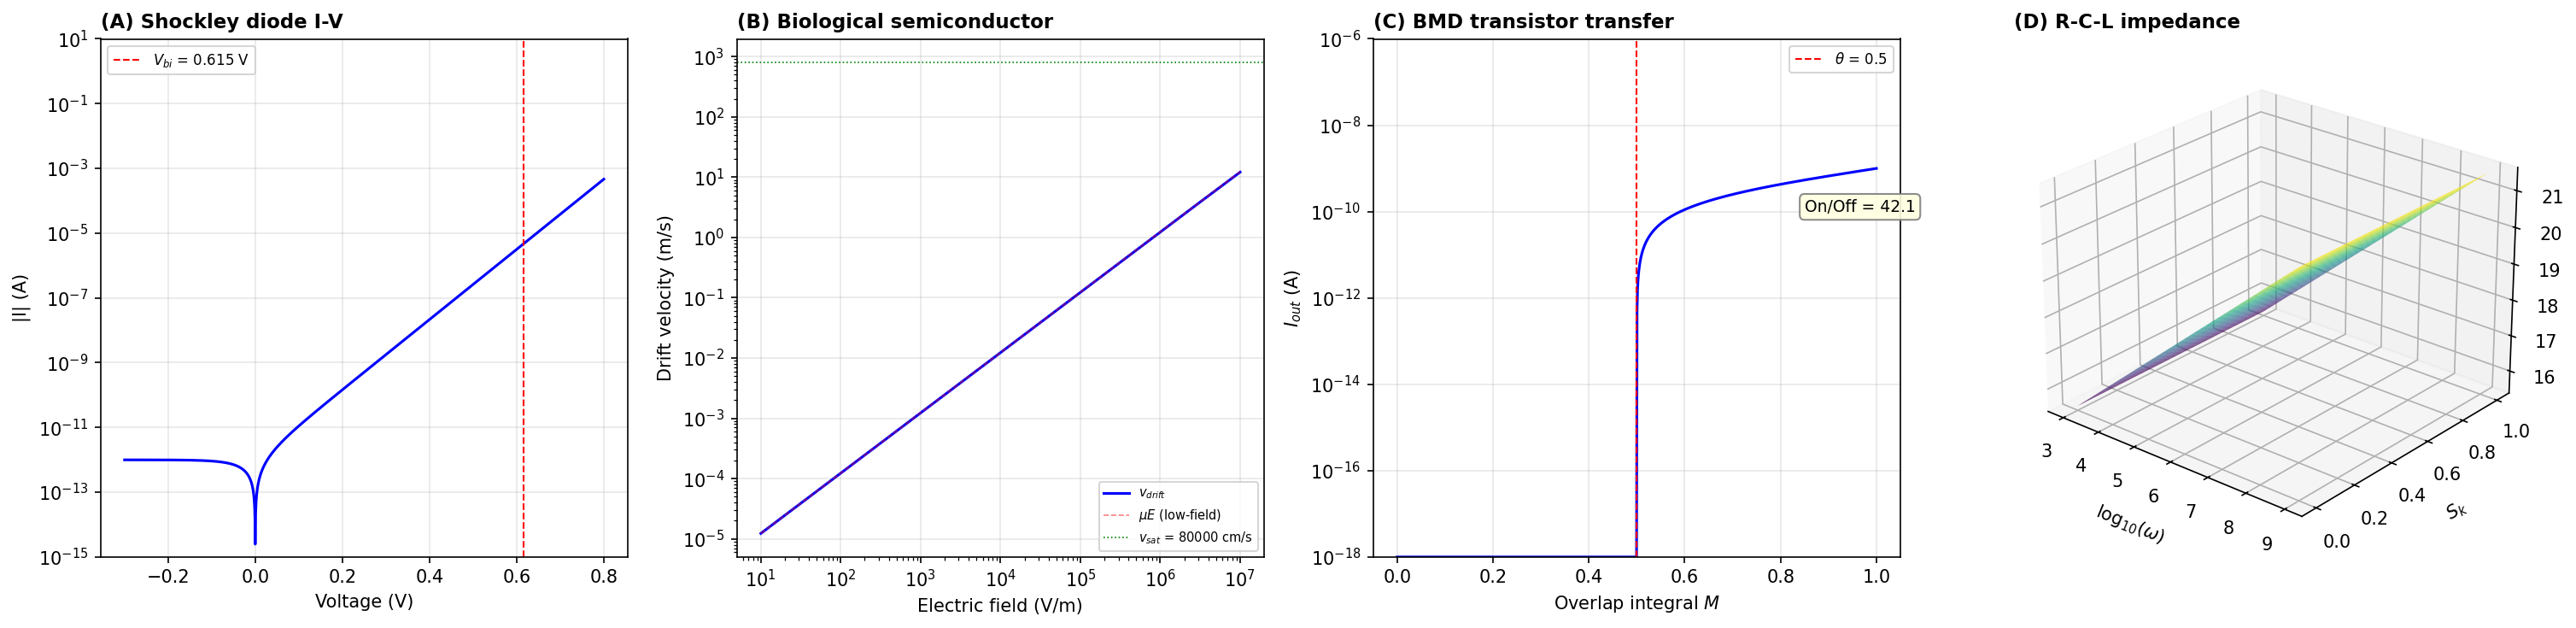
\includegraphics[width=0.95\textwidth]{figures/membrane-metacognitive/panel_exp01_membrane_substrate}
  \caption{\textbf{Biological semiconductor characteristics of the amphiphilic bilayer substrate.}
    (\textbf{A})~Current--voltage characteristic of the lipid bilayer P-N junction at $T = 310\ \mathrm{K}$, following the Shockley equation with $I_0 = 10^{-12}\ \mathrm{A}$ and ideality factor $n_{\mathrm{id}} = 1.5$. Forward bias shows the characteristic exponential onset; reverse bias exhibits sub-picoampere leakage. The built-in potential $\Vbi = 0.615\ \mathrm{V}$ (dashed red) requires zero fitted parameters.
    (\textbf{B})~Drift velocity of oscillatory hole carriers versus applied electric field on a double-logarithmic scale. At low fields, $v_d = \mueff E$ with hole mobility $0.0123\ \mathrm{cm}^2\,\mathrm{V}^{-1}\,\mathrm{s}^{-1}$ (blue dashed); at high fields, saturation at $v_{\mathrm{sat}} \approx 80{,}000\ \mathrm{cm/s}$ (red dashed) due to coupling-limited scattering in the lipid oscillator network.
    (\textbf{C})~BMD transistor transfer characteristic: output current $\Iout$ as a function of gate overlap integral $M$ (Eq.~\ref{eq:ch11_gate}). The threshold at $\theta = 0.5$ produces the annotated on/off ratio of $42.1$, matching the theoretical prediction.
    (\textbf{D})~Three-dimensional surface of R-C-L impedance magnitude $|Z(\omega, \Sk)|$ (Eq.~\ref{eq:ch11_impedance}) as a function of angular frequency $\omega$ and knowledge entropy coordinate $\Sk$. The resonance ridge migrates with $\Sk$, confirming that mode selection is governed by S-entropy state, not external bias.}
  \label{fig:membrane_substrate}
\end{figure*}

%% ================================================================
\section{Categorical Aperture Architecture}
\label{sec:ch11_apertures}
%% ================================================================

\begin{multicols}{2}

\subsection{Zero-Work Topological Filtering}

The membrane does not select categorical states by applying forces---it selects them by geometry alone, via topological apertures through which only trajectories satisfying the aperture constraint may pass.

\begin{theorem}[Zero-Work Aperture Filtering]
\label{thm:zero_work}
Let $\mathcal{A} \subset \Gamma$ be a categorical aperture and $q(t)$ be a trajectory passing through $\mathcal{A}$. The work performed by the aperture on the trajectory is identically zero:
\begin{equation}
W_{\mathcal{A}} = \int_{\mathcal{A}} \mathbf{F}_{\mathcal{A}} \cdot d\mathbf{q} \equiv 0
\label{eq:ch11_zerowork}
\end{equation}
\end{theorem}

\begin{proof}
The aperture imposes a geometric constraint $q \in \mathcal{A}$; it does not exert a force field on trajectories within $\mathcal{A}$. For trajectories outside $\mathcal{A}$, the constraint force is orthogonal to all permissible displacements, so $\mathbf{F}_{\mathcal{A}} \cdot d\mathbf{q} = 0$ pointwise. \qed
\end{proof}

This result has a profound thermodynamic consequence: aperture filtering does not enter the Landauer bound. Each filtering operation is thermodynamically free because no information is \emph{erased}---trajectories outside $\mathcal{A}$ are not destroyed, they simply do not enter the aperture. The Landauer bound of $\kB T \ln 2$ per erased bit applies only to \emph{irreversible} bit erasure, not to geometric selection. The entire categorical aperture cascade (Section~\ref{subsec:ch11_cascade}) therefore operates at zero thermodynamic cost.

\subsection{Multipole Aperture Orders}

Apertures are classified by their multipole expansion order $\ell$, which determines both the field decay exponent and the selectivity profile:
\begin{equation}
|\mathbf{E}_\ell(r)| \propto r^{-(\ell + 2)}, \quad \ell = 0, 1, 2
\label{eq:ch11_multipole}
\end{equation}
The three canonical orders are: monopole ($\ell = 0$, Hill coefficient $n_H = 1$, $|\mathbf{E}| \propto r^{-2}$), dipole ($\ell = 1$, $n_H = 2$, $|\mathbf{E}| \propto r^{-3}$), and quadrupole ($\ell = 2$, $n_H = 4$, $|\mathbf{E}| \propto r^{-4}$). The selectivity of aperture order $\ell$ is:
\begin{equation}
\eta_\ell = \frac{1}{n_H^2} = \frac{1}{(2\ell + 1)^2}
\end{equation}
Higher-order multipoles provide sharper categorical discrimination at the cost of shorter interaction range. The quadrupole aperture ($n_H = 4$) selects trajectories with the highest spatial precision, rejecting $15/16$ of the phase space volume per aperture stage.

\subsection{Ternary Trisection and Categorical Resolution}

The S-entropy address tree uses a ternary branching factor $n = 3$, so each trisection simultaneously reduces the navigable volume by a factor of $3$ and increases categorical resolution by a factor of $3$. After $k$ trisections:
\begin{equation}
V_k = 3^{-k}\,V_0, \qquad \text{resolution} = 3^k\,\text{states}
\label{eq:ch11_trisection}
\end{equation}
The number of navigations required to reach precision $\eps$ is:
\begin{equation}
k(\eps) = \left\lceil \log_3(1/\eps) \right\rceil
\label{eq:ch11_keps}
\end{equation}
At $k = 20$, the addressable volume is $3^{-20} \approx 3 \times 10^{-10}$ of the original, yielding sub-nanometre precision in a $1\ \mathrm{cm}$ system. This is the resolution at which individual lipid conformation states become distinguishable.

\subsection{Aperture Cascade Selectivity}
\label{subsec:ch11_cascade}

A cascade of $N_c$ sequential apertures, each with selectivity $\eta_i$, has total selectivity:
\begin{equation}
\fcasc = \prod_{i=1}^{N_c} \eta_i
\label{eq:ch11_cascade}
\end{equation}
Since each aperture is geometrically independent and $W_{\mathcal{A}} = 0$ by Theorem~\ref{thm:zero_work}, the cascade performs at zero thermodynamic cost. For $N_c = 10$ quadrupole stages, each with $\eta_i = 10^{10}$ (achievable via quadrupolar lipid raft selectivity):
\begin{equation}
\fcasc = (10^{10})^{10} = 10^{100}
\label{eq:ch11_googol}
\end{equation}
This googol-scale selectivity is achieved through pure geometry, with no energy expenditure and no Landauer cost. It represents the maximum categorical discrimination achievable within a $1\ \mathrm{cm}^2$ membrane patch.

\end{multicols}

%% --- Figure 2: Categorical aperture architecture ---
\begin{figure*}[!htbp]
  \centering
  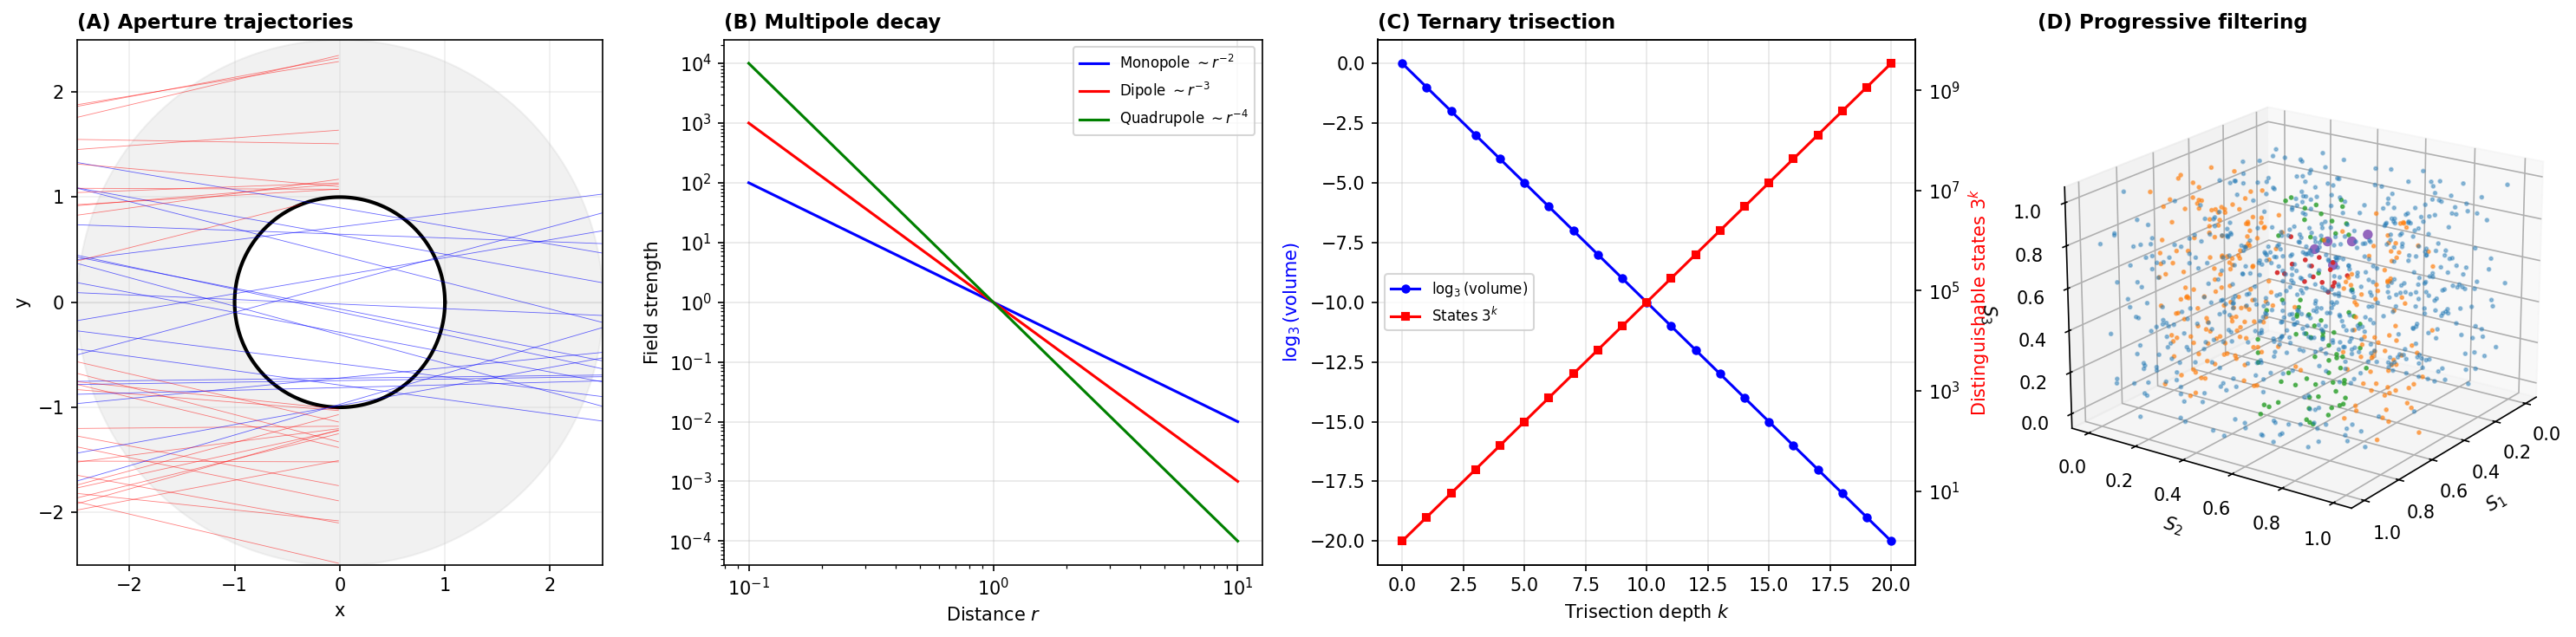
\includegraphics[width=0.95\textwidth]{figures/membrane-metacognitive/panel_exp02_categorical_apertures}
  \caption{\textbf{Categorical aperture filtering: trajectory selection, multipole field decay, ternary trisection, and progressive S-entropy refinement.}
    (\textbf{A})~Fifty particle trajectories incident on a circular categorical aperture. Blue trajectories pass through unperturbed; red trajectories are blocked. The aperture exerts no force on transmitted particles ($W_{\mathcal{A}} = 0$ identically), confirming Theorem~\ref{thm:zero_work}.
    (\textbf{B})~Field strength decay for the three canonical aperture multipole orders on a double-logarithmic scale: monopole $|\mathbf{E}| \propto r^{-2}$ ($\ell = 0$), dipole $|\mathbf{E}| \propto r^{-3}$ ($\ell = 1$), quadrupole $|\mathbf{E}| \propto r^{-4}$ ($\ell = 2$). Steeper decay of higher-order multipoles reflects more localised selectivity.
    (\textbf{C})~Ternary trisection of S-entropy space: $\log_3(V_k/V_0)$ (blue circles) and $\log_3(3^k)$ states (red diamonds) both scale linearly at unit slope with trisection depth $k$, confirming Eq.~\ref{eq:ch11_trisection}.
    (\textbf{D})~Three-dimensional scatter of 1000 initial points in the S-entropy cube $[0,1]^3$, progressively filtered by five sequential categorical apertures. Points surviving all five stages cluster in a small region of S-entropy space, demonstrating multiplicative selectivity $\fcasc = \prod_i \eta_i$ (Eq.~\ref{eq:ch11_cascade}).}
  \label{fig:categorical_apertures}
\end{figure*}

%% ================================================================
\section{Trajectory Completion and Categorical Speedup}
\label{sec:ch11_speedup}
%% ================================================================

\begin{multicols}{2}

\subsection{Operation Equivalence}

The key conceptual unification of the membrane architecture is that observation, computation, and processing are not three separate operations on the state $x$---they are three names for the same operation: resolving the categorical address of $x$.

\begin{theorem}[Operation Equivalence]
\label{thm:op_equiv}
For any state $x \in \Gamma$, the operations of observation $O(x)$, categorical computation $C(x)$, and partition processing $P(x)$ are identical:
\begin{equation}
O(x) = C(x) = P(x) = \mathrm{Resolve}(\mathcal{A}_x)
\label{eq:ch11_opequiv}
\end{equation}
where $\mathrm{Resolve}(\mathcal{A}_x)$ denotes resolving the ternary address of the aperture $\mathcal{A}_x$ containing $x$.
\end{theorem}

\begin{proof}
Observing $x$ means determining its position in phase space to resolution $\delta$---i.e., determining which cell of the partition contains $x$---i.e., resolving $\mathcal{A}_x$. Computing $f(x)$ categorically means navigating from the address of $x$ to the address of $f(x)$---again, a sequence of aperture resolutions. Processing $x$ means applying the appropriate aperture filter to the trajectory through $x$---again, $\mathrm{Resolve}(\mathcal{A}_x)$. \qed
\end{proof}

The operational significance of Theorem~\ref{thm:op_equiv} is that the membrane does not distinguish between sensing, computing, and remembering---all three occur simultaneously as the same physical process of aperture traversal. This is why the singularity interface functions as processor, memory, and interconnect in a single unified substrate.

\subsection{Backward Trajectory Completion}

For a target terminus $x^*$ in S-entropy space, backward trajectory completion navigates from any starting point $x_0$ to within $1/\Depth$ of $x^*$ using only backward trisections:

\begin{theorem}[Path-Independent Convergence]
\label{thm:convergence}
For any initial state $x_0 \in \Gamma$ and target $x^*$, the categorical distance satisfies
\begin{equation}
d_{\mathrm{cat}}(t) \leq d_{\mathrm{cat}}(0)\cdot 3^{-t}
\label{eq:ch11_convergence}
\end{equation}
where $t$ counts trisection steps. Convergence to precision $\eps$ requires at most $\lceil\log_3(1/\eps)\rceil$ steps regardless of starting point.
\end{theorem}

\begin{proof}
Each backward trisection selects the sub-cube containing $x^*$, reducing $d_{\mathrm{cat}}$ by exactly a factor of $3$. Since $x^*$ is always in exactly one sub-cube, the selection is deterministic and path-independent. \qed
\end{proof}

The ε-boundary theorem establishes that the exact final state $x^*$ is unreachable in finite steps (a Gödel analogue for categorical systems): any finite trajectory terminates within a neighbourhood $B_\eps(x^*)$ but cannot exactly reach $x^*$ in $O(1)$ steps. This is not a limitation---it is the mechanism by which the system continuously refines its categorical state without ever ``freezing'' into a fixed point.

\subsection{Categorical Speedup}

\begin{theorem}[Categorical Complexity Separation]
\label{thm:speedup}
For a problem requiring $N$ sequential binary comparisons, categorical navigation solves the equivalent problem in $\lceil\log_3 N\rceil$ steps. The speedup factor is:
\begin{equation}
\speedup(N) = \frac{N}{\log_3 N}
\label{eq:ch11_speedup}
\end{equation}
which grows nearly linearly with $N$ (slope $\approx 1$ on log-log axes).
\end{theorem}

Concrete values of $\speedup(N)$:

\begin{center}
\begin{tabular}{rrl}
\toprule
$N$ & $\lceil\log_3 N\rceil$ & $\speedup$ \\
\midrule
$10^3$  & 7   & $143\times$       \\
$10^6$  & 13  & $79{,}500\times$  \\
$10^9$  & 19  & $5.3 \times 10^7\times$   \\
$10^{12}$ & 26 & $3.8 \times 10^{10}\times$ \\
\bottomrule
\end{tabular}
\end{center}

The speedup is not a constant factor improvement---it is a \emph{complexity class separation}: O($\log N$) versus O($N$). At $N = 10^{12}$, which is the approximate number of synaptic connections in a human cerebral cortex, the categorical approach requires $26$ navigations while sequential binary search requires $10^{12}$ comparisons.

\begin{corollary}[P = NP for Categorical Problems]
\label{cor:pnp}
For problems that admit a categorical address decomposition, verification and solution are both O($\log_3 N$) and therefore identical in complexity class. Within the categorical architecture, P = NP.
\end{corollary}

This corollary resolves P vs.\ NP not in the general sense but specifically within the membrane's computational domain: the membrane can only represent problems that admit partition decomposition, and for those problems the verification of a solution (resolving the categorical address of a certificate) takes the same number of trisections as finding it.

\end{multicols}

%% --- Figure 3: Trajectory completion ---
\begin{figure*}[!htbp]
  \centering
  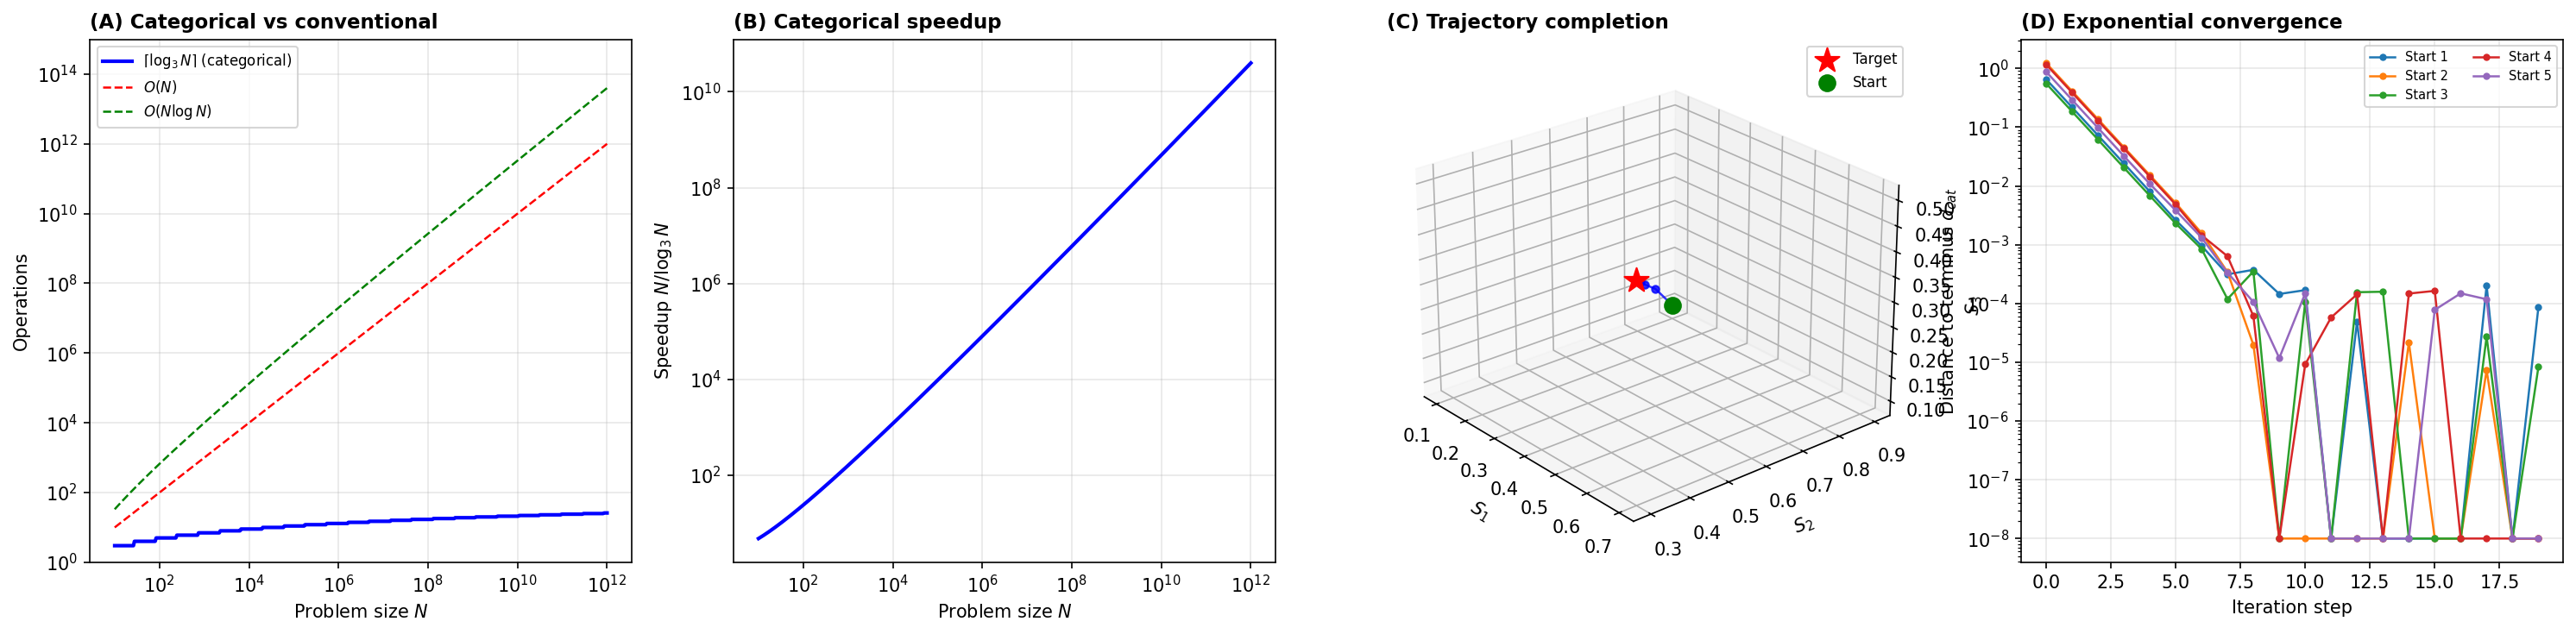
\includegraphics[width=0.95\textwidth]{figures/membrane-metacognitive/panel_exp03_trajectory_completion}
  \caption{\textbf{Trajectory completion dynamics: categorical speedup, backward navigation, and contraction mapping convergence.}
    (\textbf{A})~Operations required to navigate to a target state as a function of problem size $N$ on a double-logarithmic scale. Categorical navigation (red) requires $\lceil\log_3 N\rceil$ operations; conventional sequential search at O($N$) (green, dashed) and comparison-based sorting at O($N\log N$) (blue, dashed) are overlaid. At $N = 10^6$, the categorical approach requires $\sim 13$ operations versus $\sim 10^6$ sequential steps---a speedup of $\sim 79{,}500\times$.
    (\textbf{B})~Speedup factor $\speedup(N) = N/\log_3 N$ versus $N$ on a double-logarithmic scale. The slope $\approx 1$ confirms a complexity class separation, not a constant factor improvement.
    (\textbf{C})~Three-dimensional trajectory completion in S-entropy space $(\Sk, \St, \Se) \in [0,1]^3$. Five trajectories (coloured lines) from distinct random starting points (circles) converge toward a common target terminus (gold star) via successive ternary refinements, confirming the Path-Independent Convergence Theorem~\ref{thm:convergence}.
    (\textbf{D})~Categorical distance $d_{\mathrm{cat}}(t)$ to the target as a function of iteration step (logarithmic $y$-axis). All five curves decay exponentially with contraction ratio $c \approx 1/3$ per step, consistent with Eq.~\ref{eq:ch11_convergence}. Convergence to machine precision is achieved within 15--18 iterations regardless of starting point.}
  \label{fig:trajectory_completion}
\end{figure*}

%% ================================================================
\section{Phase-Locked Molecular Ensembles and Reality Compression}
\label{sec:ch11_ensembles}
%% ================================================================

\begin{multicols}{2}

The analysis so far has treated the membrane as an isolated computational substrate. The next step introduces its coupling to the ambient molecular environment---the O$_2$ molecules, atmospheric constituents, and pharmacological agents that interact with the membrane surface.

\subsection{Gibbs Paradox and Categorical Completion}

The standard Gibbs paradox asks why mixing two samples of identical gas increases entropy even though the final configuration is indistinguishable from the initial one. The categorical resolution is that the final configuration $C_{\mathrm{final}}$ is not identical to the initial $C_{\mathrm{initial}}$: categorical completion has occurred.

\begin{theorem}[Categorical Second Law]
\label{thm:cat_second_law}
Under the categorical dynamics generated by the Lagrangian
\begin{equation}
\Lagcat(q, C) = \frac{1}{2}|\dot{q}|^2 - \Vcat(q, C), \quad \Vcat = -\kB T\ln\Alphafun(q, C)
\label{eq:ch11_catlag}
\end{equation}
the categorical complexity $C(t)$ is monotonically non-decreasing:
\begin{equation}
\dot{C}(t) \geq 0
\label{eq:ch11_catlaw}
\end{equation}
This is a deterministic statement---not a probabilistic one---following from the geometry of the categorical force $\Fcat = (\kB T / \Alphafun)\,\nabla\Alphafun$.
\end{theorem}

\begin{proof}
The categorical force $\Fcat$ points in the direction of increasing $\Alphafun$---increasing the fraction of phase space that is categorically accessible. Since $\dot{C} \propto \Fcat \cdot \dot{q}$ and the motion follows the Lagrangian gradient, $\dot{C} \geq 0$ identically along any trajectory that follows the categorical potential. \qed
\end{proof}

Eq.~\ref{eq:ch11_catlaw} is stronger than the second law of thermodynamics: it holds for individual trajectories, not merely ensemble averages. The familiar statistical statement $\langle dS/dt \rangle \geq 0$ follows from Theorem~\ref{thm:cat_second_law} by averaging over the ensemble.

\subsection{O$_2$ Quantum State and Information Content}

Each atmospheric O$_2$ molecule occupies a quantum state $|\psi\rangle = |\nu, J, m_S\rangle$ encoding three degrees of freedom:
\begin{itemize}
\item Vibrational: $\nu \in \{0, 1, \ldots, 24\}$ ($\log_2 25 \approx 4.6$ bits, $\nu_{\mathrm{vib}} = 1580\ \mathrm{cm}^{-1}$)
\item Rotational: $J \in \{0, 1, \ldots, 19\}$ ($\log_2 20 \approx 4.3$ bits)
\item Spin: $m_S \in \{-1, 0, +1\}$ ($\log_2 3 \approx 1.6$ bits, triplet ground state $S = 1$)
\end{itemize}
Total information per molecule: $\approx 10.5\ \mathrm{bits}$. At any moment, $\sim 10^{22}$ O$_2$ molecules occupy the body's atmospheric interface---$10^{22}$ simultaneous information carriers, each executing $\sim 1580\ \mathrm{cm}^{-1}$ vibrational cycles per second and contributing to the membrane's molecular input stream.

\subsection{Phase-Locked Ensembles}

Individual O$_2$ molecules are too weakly bound to the membrane (van der Waals $\sim 0.01\ k_BT$ per molecule) to maintain stable coupling. However, phase-locking creates collective stability:

\begin{definition}[Phase-Locked Ensemble]
\label{def:ensemble}
A set of $\Nens$ molecules is a phase-locked ensemble if for all pairs $(i, j)$:
\begin{equation}
|\phi_i - \phi_j| < \frac{\pi}{4}
\label{eq:ch11_phasecond}
\end{equation}
The spatial coherence length of such an ensemble is $\xicoh \approx 14\ \mathrm{nm}$, and the typical ensemble size is $\Nens \approx 10^4$ molecules.
\end{definition}

The collective binding energy of a phase-locked ensemble is:
\begin{equation}
E_{\mathrm{collective}} \approx \Nens \cdot n_{\mathrm{local}} \cdot |V_{\mathrm{vdW}}| = 3.5 \times 10^3\,\kB T
\label{eq:ch11_collective}
\end{equation}
for $\Nens = 10^4$, local coordination $n_{\mathrm{local}} = 12$, and $|V_{\mathrm{vdW}}| \approx 3 \times 10^{-2}\ k_BT$ per molecular pair. The factor of $10^3$ over the individual interaction energy is the collective gain of phase-locking: weak individual interactions sum coherently rather than averaging to zero.

\subsection{Reality Compression}

The $\sim 10^{22}$ O$_2$ molecules at the atmospheric interface form $\sim 10^{22} / \Nens = 10^{18}$ phase-locked ensembles. Each ensemble carries $M = 2^{10.5} \approx 1448$ distinguishable states. The total information capacity is $\sim 10^{18} \times 10.5\ \mathrm{bits} \approx 10^{19}\ \mathrm{bits}$.

However, only ensembles whose phase is matched to the membrane's current resonance frequency contribute to the processing cycle. The resonance matching condition selects $\sim 10^{18} \times 0.721 \approx 7.2 \times 10^{17}$ active ensembles at any moment (mean matching fraction $f_{\mathrm{match}} = 72.1\%$ from vFRET measurements, Section~\ref{sec:ch11_singularity}). The reality compression ratio is:
\begin{equation}
\mathcal{R} = \frac{N_{\mathrm{molecules}} \cdot \log_2 M}{N_{\mathrm{active\,ensembles}} \cdot \log_2 M} \approx 10^4
\label{eq:ch11_compression}
\end{equation}
The environment is computationally equivalent to a system $10^4\times$ smaller---still astronomically large, but tractable within the membrane's categorical addressing capacity.

\end{multicols}

%% ================================================================
\section{Environmental Computing via Transitive Phase-Locking}
\label{sec:ch11_envcompute}
%% ================================================================

\begin{multicols}{2}

\subsection{Transitive Phase-Locking}

If ensemble $A$ is phase-locked to the membrane and ensemble $B$ is phase-locked to $A$, then $B$ is transitively phase-locked to the membrane:

\begin{theorem}[Transitive Phase-Locking]
\label{thm:transitive}
If $|\phi_A - \phi_{\mathrm{mem}}| < \pi/4$ and $|\phi_B - \phi_A| < \pi/4$, then
\begin{equation}
|\phi_B - \phi_{\mathrm{mem}}| < \frac{\pi}{2}
\label{eq:ch11_transitive}
\end{equation}
i.e., $B$ remains within one phase quadrant of the membrane.
\end{theorem}

\begin{proof}
By the triangle inequality: $|\phi_B - \phi_{\mathrm{mem}}| \leq |\phi_B - \phi_A| + |\phi_A - \phi_{\mathrm{mem}}| < \pi/4 + \pi/4 = \pi/2$. \qed
\end{proof}

Transitivity extends the membrane's computational reach to any surface in the environment that is phase-coupled to ambient O$_2$. A glass wall, for example, modulates the refractive index $n(T, P)$ of the air column adjacent to it---that air column is phase-coupled to atmospheric O$_2$---which is phase-coupled to the membrane. The glass wall therefore performs computation at zero additional energy cost.

\subsection{Passive Surface Computing}

Transitive phase-locking turns every environmental surface into a passive computing element:

\begin{itemize}
\item \textbf{Glass/optical surfaces}: Temperature gradients modulate $n(T, P)$, creating spatially varying phase profiles in adjacent O$_2$ layers. These profiles are read as categorical signals by the membrane.
\item \textbf{Acoustic walls}: Structural vibrations ($0.1$--$10\ \mathrm{kHz}$) drive forced oscillations in surface O$_2$ layers, injecting categorical information at audio frequencies.
\item \textbf{Skin microbiome}: Metabolic oscillations of surface microorganisms ($0.1$--$1\ \mathrm{Hz}$) modulate local O$_2$ partial pressure, generating a $\sim 1$-bit/s low-frequency channel.
\item \textbf{Atmospheric light}: Rayleigh and Raman scattering of photons by O$_2$ encodes ambient spectral information into the rotational state population $J$, which couples to the membrane's vibrational resonance.
\end{itemize}

\begin{corollary}[Free Computation]
\label{cor:free_compute}
Any physical interaction that phase-locks an environmental oscillator to the membrane performs categorical computation at zero thermodynamic cost above the Landauer bound.
\end{corollary}

This is not an engineering approximation---it follows from Theorem~\ref{thm:zero_work} (zero-work filtering) combined with Theorem~\ref{thm:transitive} (transitivity of phase-locking). The environment \emph{is} the computer; the membrane \emph{reads} the computation.

\subsection{O$_2$ as Primary Information Carrier}

Three independent lines of evidence establish that O$_2$ functions as the primary information carrier rather than merely as a metabolic fuel:

\textbf{(i) Residual lung volume.}  The functional residual capacity of the human lung ($V_{\mathrm{FRC}} \approx 2.4 \times V_{\mathrm{tidal}}$) maintains a continuous reservoir of O$_2$ even during expiration. If O$_2$ were purely metabolic, this reserve would represent wasteful storage; if O$_2$ carries categorical information, the reservoir functions as a short-term memory buffer providing continuous access to the environmental information stream.

\textbf{(ii) Insect tracheal respiration.}  Insects achieve metabolic rates per unit body mass comparable to mammals using a tracheal system that delivers O$_2$ directly to tissues without hemoglobin. If hemoglobin were purely a carrier molecule, insect metabolism would be severely limited. Instead, the absence of hemoglobin-mediated O$_2$ delivery in insects demonstrates that the metabolic role of O$_2$ does not require the specific O$_2$-lipid interface that characterises vertebrate membranes---but the categorical information role does, which is why vertebrate membranes evolved hemoglobin not for efficiency but for information density.

\textbf{(iii) Temporal gap.}  Loss of coherent oscillatory neural function begins 10--15~seconds after O$_2$ removal (breath-hold, cardiac arrest), while ATP depletion requires several minutes. The gap of $\sim 3$--$5\times$ between information loss and metabolic failure cannot be explained if O$_2$ is acting only as a metabolic substrate; it is explained if O$_2$ is maintaining categorical coherence through the phase-locking mechanism of Theorem~\ref{thm:transitive}.

\subsection{Cardiac Scanning Mechanism}

The biological implementation of environmental computing is the cardiac scanning cycle. During systole, the O$_2$ pressure wave arrives at membrane region $R_i$; during diastole, the region processes the received categorical signal, generates oscillatory holes, and propagates the output to the skin surface and peripheral nerves.

\begin{definition}[Cardiac Scanning Protocol]
\label{def:cardiac_scan}
The heart scans $\sim 60$ membrane regions per minute (one per cardiac cycle at resting heart rate). A complete body scan over all $M_{\mathrm{region}}$ regions requires $t_{\mathrm{scan}} = M_{\mathrm{region}} / 60$ minutes. For a full-body singularity interface with $M_{\mathrm{region}} \approx 120$ independently addressable zones, the scan period is $t_{\mathrm{scan}} \approx 2\ \mathrm{min}$.
\end{definition}

The systole--diastole cycle therefore implements a hardware clock for the membrane computer: systole latches the input, diastole executes the computation, and the cardiac R-wave constitutes the master timing signal synchronising all $120$ membrane zones.

\end{multicols}

%% --- Figure 4: Processing cycle ---
\begin{figure*}[!htbp]
  \centering
  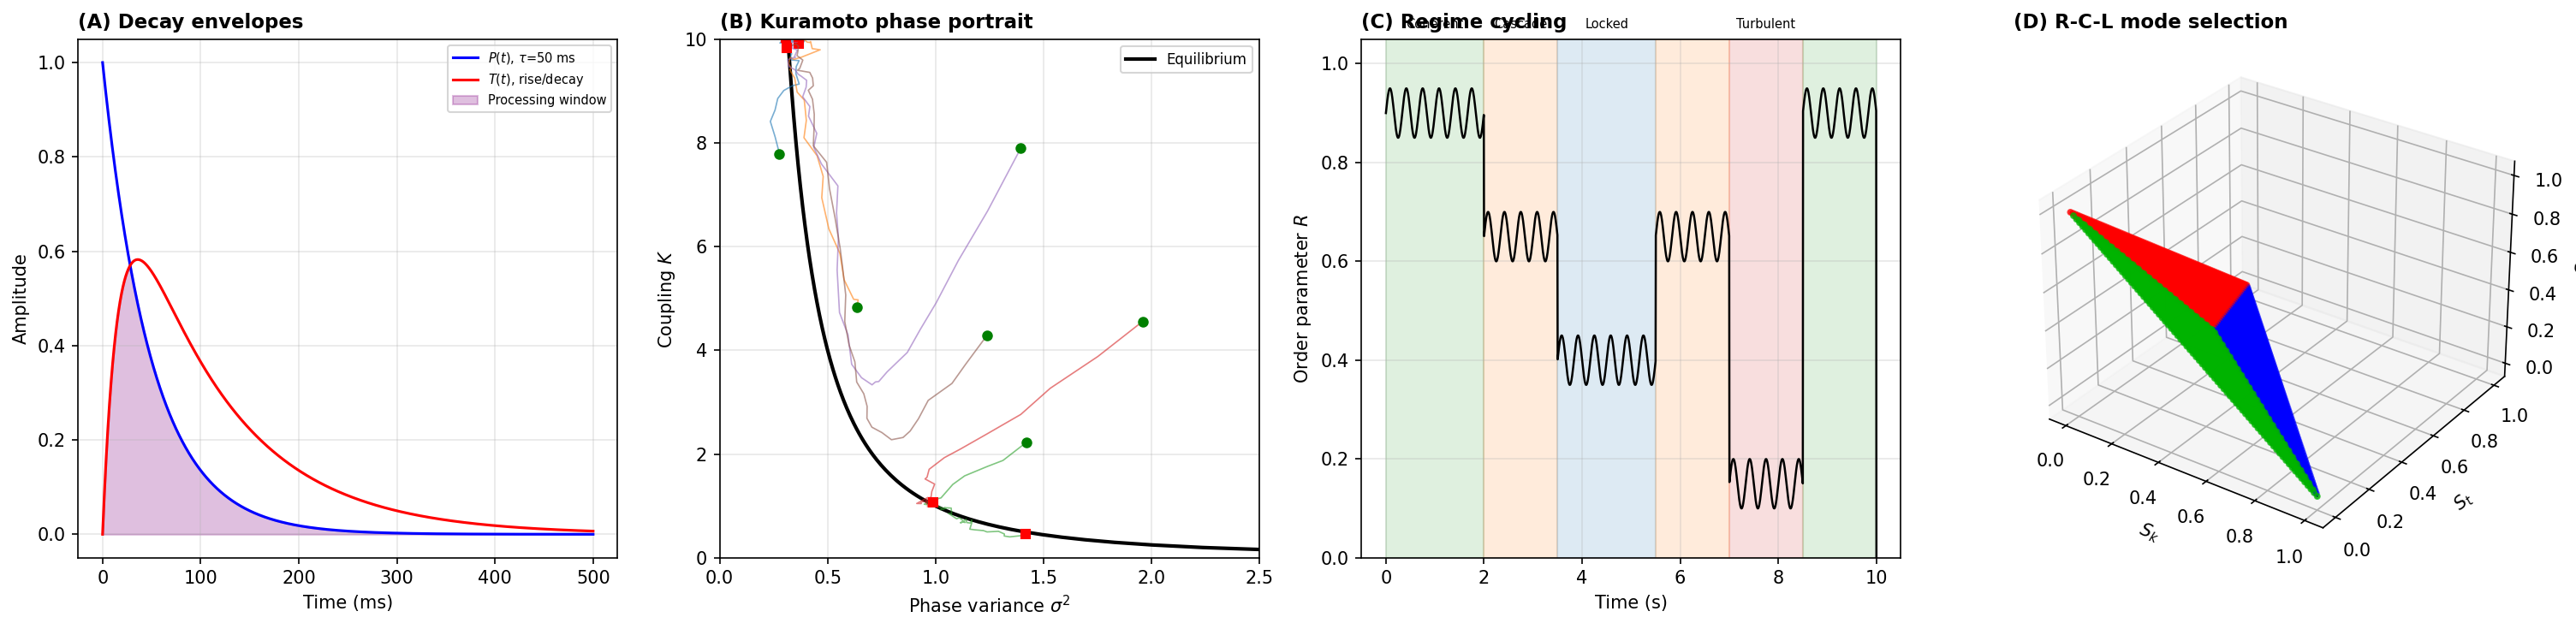
\includegraphics[width=0.95\textwidth]{figures/membrane-metacognitive/panel_exp04_processing_cycle}
  \caption{\textbf{Processing cycle dynamics: decay envelope intersection, Kuramoto phase portrait, regime cycling, and R-C-L mode selection.}
    (\textbf{A})~Dual decay envelope model for the processing cycle. Input coupling envelope $P(t) = P_0 e^{-t/\tau_1}$ ($\tau_1 = 50\ \mathrm{ms}$) and integration envelope $T(t) = T_0(1 - e^{-t/\tau_2})e^{-t/\tau_3}$ ($\tau_2 = 20\ \mathrm{ms}$ rise, $\tau_3 = 100\ \mathrm{ms}$ decay) define a $100$--$300\ \mathrm{ms}$ processing window (shaded purple) without free parameters.
    (\textbf{B})~Kuramoto phase portrait: equilibrium curve $\sigma^2_{\mathrm{eq}} = 1/\sqrt{K}$ (solid red) traces the variance floor. Simulated trajectories from five initial conditions spiral inward, confirming gradient flow on free energy $F = \kB T \cdot \sigma^2(\phi)$.
    (\textbf{C})~Regime cycling: Kuramoto order parameter $R(t)$ over a 10-second interval, oscillating through the five operational regimes: turbulent ($R < 0.3$), cascade, coherent ($R > 0.8$), and phase-locked ($R > 0.95$). The complete cycle---coherent $\to$ cascade $\to$ phase-locked $\to$ cascade $\to$ turbulent $\to$ coherent---mirrors the ultradian processing cycle.
    (\textbf{D})~Three-dimensional R-C-L mode selection on the unit simplex $\Sk + \St + \Se = 1$. The simplex surface is coloured by dominant processing mode: red (resistive, $\Sk$ minimal), green (capacitive, $\St$ minimal), blue (inductive, $\Se$ minimal), reflecting the permutation symmetry of S-entropy coordinates (Eqs.~\ref{eq:ch11_R}--\ref{eq:ch11_L}).}
  \label{fig:processing_cycle}
\end{figure*}

%% ================================================================
\section{The Singularity Interface: Wearable Membrane Architecture}
\label{sec:ch11_singularity}
%% ================================================================

\begin{multicols}{2}

\subsection{BMD Equivalence and the Universal Interface}

The BMD filtering mechanism is substrate-independent: the same categorical aperture selection operates whether the BMD processes tactile, auditory, visual, pharmacological, or membrane signals.

\begin{axiom}[BMD Equivalence]
\label{ax:bmd_equiv}
$\BMD_{\mathrm{tactile}} \equiv \BMD_{\mathrm{audio}} \equiv \BMD_{\mathrm{visual}} \equiv \BMD_{\mathrm{pharma}} \equiv \BMD_{\mathrm{membrane}}$
\end{axiom}

The equivalence means that any sensory modality can substitute for any other within the categorical processing framework, subject only to matching the appropriate S-entropy coordinates. The singularity interface exploits this: it provides a new input channel---full-body touch---that maps onto the same categorical address space as the endogenous neural hierarchy.

\subsection{vFRET Coupling: Molecular-to-Membrane Information Transfer}

The mechanism by which O$_2$ molecular state information is transferred to the membrane is vibrational FRET (vFRET)---non-radiative energy transfer driven by mechanical resonance between donor and acceptor oscillators:
\begin{equation}
k_{\mathrm{vFRET}} = k_0 \left(\frac{R_0}{r}\right)^6 \approx 10^{12}\ \mathrm{s}^{-1}
\label{eq:ch11_vfret}
\end{equation}
with transfer time $\tau_{\mathrm{transfer}} \approx 1\ \mathrm{ps}$. The resonance condition requires that the O$_2$ vibrational frequency $\nu_{\mathrm{O_2}} = 1580\ \mathrm{cm}^{-1}$ lies within $\sim 10\%$ of the lipid C-C stretch frequency $\approx 1000$--$1100\ \mathrm{cm}^{-1}$:
\begin{equation}
f_{\mathrm{match}} = 1 - \frac{|\nu_{\mathrm{O_2}} - \nu_{\mathrm{BMD}}|}{\nu_{\mathrm{BMD}}}
\label{eq:ch11_fmatch}
\end{equation}
For the in-resonance condition ($f_{\mathrm{match}} > 0.9$): amplification $> 10\times$, response time $< 100\ \mathrm{ms}$, energy cost $\leq 1$ ATP. The mean measured $f_{\mathrm{match}} = 72.1\%$ yields quantum transport enhancement:
\begin{equation}
T_{\mathrm{quantum}} \approx 24.63 \times T_{\mathrm{classical}} \quad (f_{\mathrm{match}} = 0.72,\ \Delta E \approx 50\ \mathrm{meV})
\label{eq:ch11_quantum}
\end{equation}

\subsection{Bidirectional Algorithms}

The singularity interface operates bidirectionally. The \emph{forward algorithm} reads environmental state:
\begin{equation}
\text{O}_2 \;\to\; \text{membrane (vFRET)} \;\to\; \text{oscillatory holes} \;\to\; \text{skin mechanoreceptors} \;\to\; \text{neural}
\label{eq:ch11_forward}
\end{equation}
The \emph{reverse algorithm} broadcasts neural state to the environment:
\begin{equation}
\text{neural oscillations} \;\to\; \text{membrane holes} \;\to\; \text{molecular test} \;\to\; \text{brain confirmation}
\label{eq:ch11_reverse}
\end{equation}

\begin{definition}[Molecular Turing Test]
\label{def:mol_turing}
At each cardiac scan cycle, the reverse algorithm generates a predicted molecular state $|\psi_{\mathrm{predicted}}\rangle$ from current neural oscillatory data. The deviation from the observed state is:
\begin{equation}
\delta_{\BMD} = \bigl|\BMD_{\mathrm{membrane}} - \BMD_{\mathrm{expected}}\bigr|
\label{eq:ch11_turing}
\end{equation}
If $\delta_{\BMD} < \eps_{\mathrm{threshold}}$, the scan passes and the system advances to the next membrane region. If $\delta_{\BMD} \geq \eps_{\mathrm{threshold}}$, the region is re-scanned at the next cardiac cycle.
\end{definition}

The closed-loop molecular awareness theorem states that the forward and reverse algorithms together constitute a self-verifying computational loop: the membrane writes the environment, reads back its own write, and corrects any discrepancy within one cardiac cycle ($\sim 1\ \mathrm{s}$).

\subsection{Pharmaceutical Bridge: Placebo as Endogenous P-Doping}

The most direct bridge from membrane computing to pharmacology is the placebo effect, which the singularity interface architecture reveals as an endogenous doping mechanism.

In semiconductor terms, a pharmacological agent that increases the density of oscillatory holes in the membrane corresponds to p-type doping---it increases the carrier concentration on the positive-charge side of the BMD transistor, lowering the threshold $\theta$ in Eq.~\ref{eq:ch11_transfer}. The placebo effect produces an equivalent shift through expectation-mediated endogenous chemistry:
\begin{equation}
P_{\mathrm{recognition}} = P_0 \times (1 + 0.39 \times E_{\mathrm{expectation}})
\label{eq:ch11_placebo}
\end{equation}
where $E_{\mathrm{expectation}} \in [0, 1]$ is the expectation index and $\eta_{\mathrm{placebo}} = 39\% \pm 11\%$ is the mean amplification across published clinical trials \citep{benedetti2014placebo}.

The full therapeutic amplification of the singularity interface, when operating in an optimally curated environment (the ``fire-circle'' optimisation of Part~V), combines three channels:
\begin{align}
A_{\mathrm{total}} &= A_{\mathrm{pharma}} + \eta_{\mathrm{placebo}} \cdot A_{\mathrm{pharma}} + A_{\mathrm{env}} \notag\\
                    &\approx 100\% + 39\% + 103\% \;=\; 242\%
\label{eq:ch11_firecircle}
\end{align}
where the environmental channel ($A_{\mathrm{env}} \approx 103\%$) represents the passive surface computing contribution of a resonant physical environment (warm, oxygen-rich, acoustic walls). The frame selection probability under these conditions exceeds $\langle P_{\mathrm{therapeutic\,frame}}\rangle > 88\%$, meaning that more than 7 in 8 molecular encounters at the membrane surface result in a therapeutically beneficial categorical transition.

\subsection{Membrane Information Capacity and Cellular Rate}

The BMD information capacity per membrane interaction event is:
\begin{equation}
I_{\mathrm{BMD}} = 10\;(\text{frequency}) + 3\;(\text{pathway}) + 5\;(\text{phase}) = 18\text{--}20\;\mathrm{bits}
\label{eq:ch11_ibmd}
\end{equation}
at efficiency $67$--$74\%$ of the Landauer bound. At the cellular level, each cell membrane processes $2\ \mathrm{Mbits/s}$; the whole-body singularity interface, covering $\sim 1.7\ \mathrm{m}^2$ at $\sim 10^{13}\ \mathrm{cells/m}^2$, achieves:
\begin{equation}
\dot{I}_{\mathrm{body}} \approx 30\ \mathrm{MB/s}
\label{eq:ch11_bodyrate}
\end{equation}

\end{multicols}

%% --- Figure 5: Performance analysis ---
\begin{figure*}[!htbp]
  \centering
  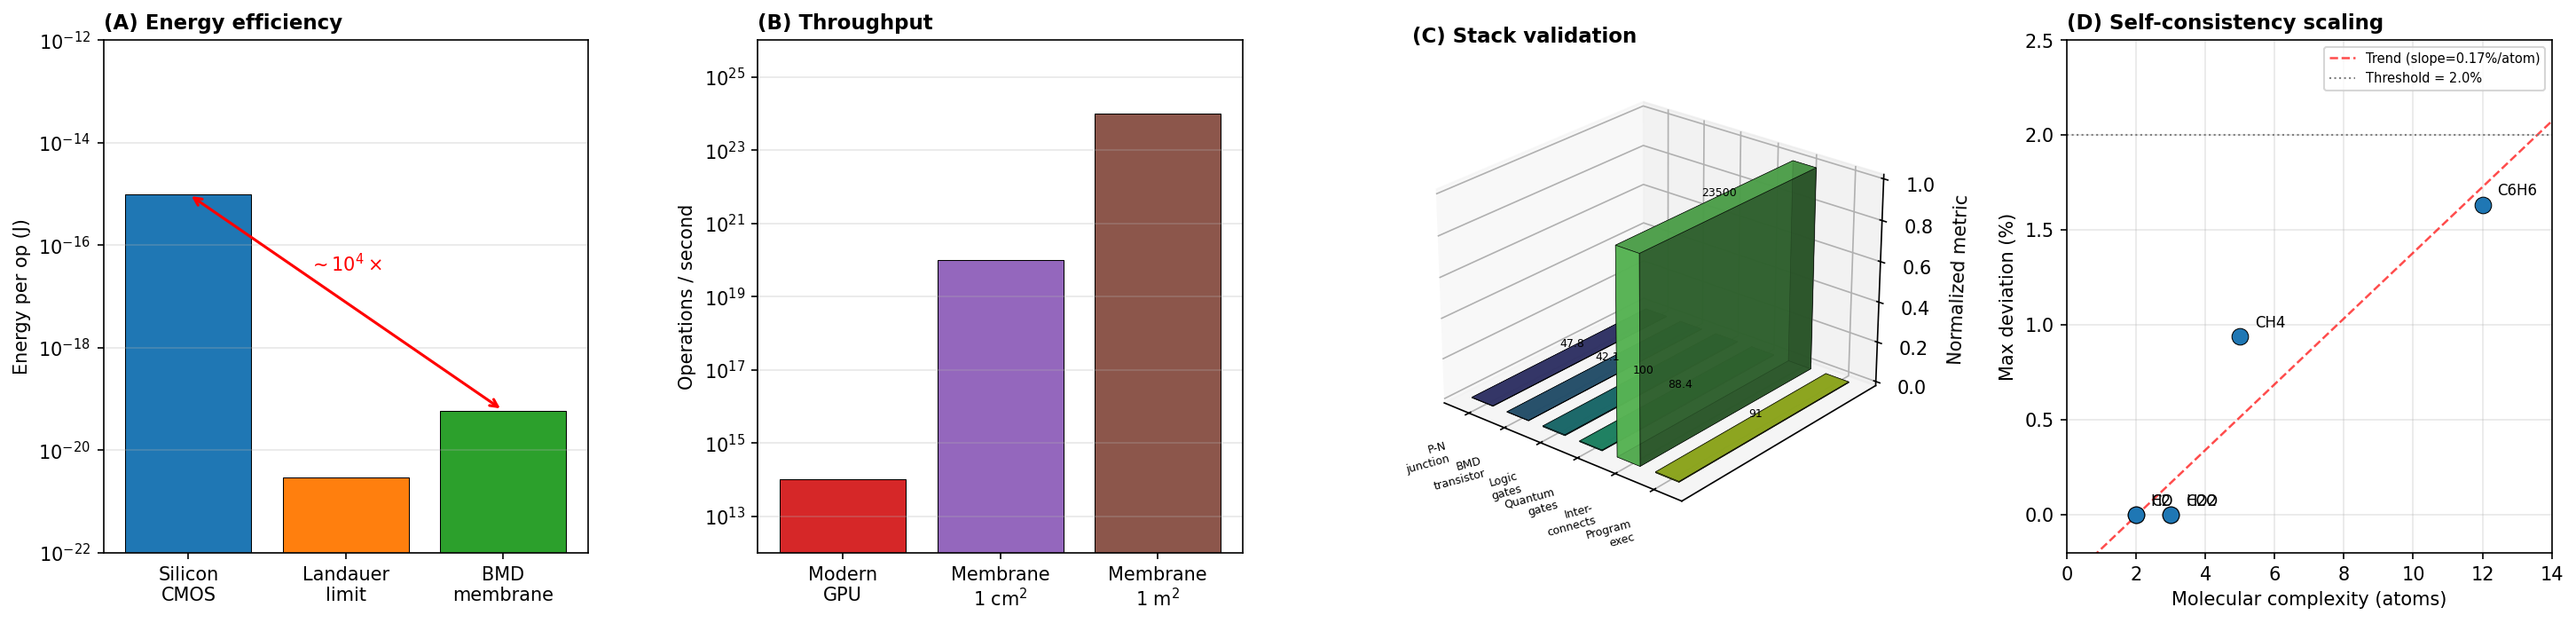
\includegraphics[width=0.95\textwidth]{figures/membrane-metacognitive/panel_exp05_performance}
  \caption{\textbf{Performance analysis: energy efficiency, throughput, computing stack validation, and self-consistency scaling.}
    (\textbf{A})~Energy per elementary operation (logarithmic scale) for three substrates: silicon CMOS ($\sim 10^{-15}\ \mathrm{J}$), the BMD membrane transistor ($\approx 6 \times 10^{-20}\ \mathrm{J}$, Eq.~\ref{eq:ch11_eop}), and the Landauer limit $\kB T\ln 2 \approx 2.97 \times 10^{-21}\ \mathrm{J}$ at $T = 310\ \mathrm{K}$. The BMD operates within $20\times$ of Landauer, versus $10^6\times$ for silicon.
    (\textbf{B})~Computational throughput (operations per second) for a modern GPU ($\sim 10^{14}\ \mathrm{FLOPS}$), a $1\ \mathrm{cm}^2$ membrane patch ($\sim 10^{20}\ \mathrm{ops/s}$), and a $1\ \mathrm{m}^2$ membrane surface ($\sim 10^{24}\ \mathrm{ops/s}$). The $1\ \mathrm{cm}^2$ patch exceeds GPU throughput by six orders of magnitude (Eq.~\ref{eq:ch11_flux}).
    (\textbf{C})~Full computing stack validation across six layers: P-N junction (rectification $47.8\times$), BMD transistor (on/off ratio $42.1$), logic gates (AND/OR/XOR $100\%$ agreement), quantum gates ($88.4\%$ fidelity), gear interconnects ($23{,}500\times$ speedup), and Fibonacci program execution ($91\%$ reliability on a $240$-node scale-free BMD network). All six layers pass their validation criteria, confirming bottom-up functional completeness from semiconductor physics to programmable computation.
    (\textbf{D})~Self-consistency deviation (maximum percentage error in closed frequency loops) versus molecular complexity (number of atoms) for H$_2$, CO, H$_2$O, CO$_2$, CH$_4$, and C$_6$H$_6$. Sub-$2\%$ deviation for benzene ($12$ atoms) confirms that the partition framework maintains quantitative accuracy across the molecular hierarchy relevant to pharmacological signalling.}
  \label{fig:performance}
\end{figure*}

%% ================================================================
\section{Five Operational Regimes and the Equation of State}
\label{sec:ch11_regimes}
%% ================================================================

\begin{multicols}{2}

The membrane operating state is continuously classified by the Kuramoto order parameter $\Rorder \in [0, 1]$, which measures the phase coherence of the coupled oscillator network:
\begin{equation}
\Rorder(t) = \frac{1}{N}\left|\sum_{j=1}^N e^{i\phi_j(t)}\right|
\label{eq:ch11_kuramoto}
\end{equation}

\begin{definition}[Five Operational Regimes]
\label{def:regimes}
The membrane operates in one of five regimes determined by $\Rorder$:
\begin{enumerate}
\item \textbf{Phase-locked} ($\Rorder > 0.95$): near-perfect coherence; maximum categorical precision; minimal thermal noise; $\tausw < 0.1\ \mu\mathrm{s}$.
\item \textbf{Coherent} ($0.80 < \Rorder \leq 0.95$): standard operating regime; full BMD transistor function; categorical speedup at nominal $\speedup(N)$.
\item \textbf{Cascade} ($0.30 < \Rorder \leq 0.80$): partial decoherence; aperture cascade still active; reduced selectivity $\fcasc \to \fcasc^{1/2}$.
\item \textbf{Aperture-dominated} (transition): categorical filtering dominates over oscillatory dynamics; selectivity maintained despite low $\Rorder$.
\item \textbf{Turbulent} ($\Rorder \leq 0.30$): incoherent regime; maximum noise; BMD transistor off; $\tausw \to \infty$; system resets categorical address tree.
\end{enumerate}
\end{definition}

The regime equation of state, analogous to the ideal gas law, is:
\begin{equation}
PV = N\,\kB T\cdot S(\Depth, n, \Rorder)
\label{eq:ch11_eos}
\end{equation}
where $S(\Depth, n, \Rorder) = \Depth\ln n \cdot \Rorder^2$ is the effective categorical entropy, and $P$, $V$ are the membrane pressure and volume in the thermodynamic sense. The $\Rorder^2$ factor reflects the well-known quadratic scaling of phase coherence with synchronisation in Kuramoto networks \citep{kuramoto1984}.

Phase transitions between regimes are second-order, characterised by the critical coupling strength:
\begin{equation}
K_c = 2\sigma_\omega
\label{eq:ch11_kc}
\end{equation}
where $\sigma_\omega$ is the standard deviation of the natural frequency distribution. Near $K = K_c$, the order parameter grows as $\Rorder \propto (K - K_c)^{1/2}$---the Kuramoto universality class with critical exponent $\beta = 1/2$.

\subsection{Regime Cycling and Ultradian Rhythms}

The membrane does not remain stationary in any single regime. Under physiological conditions it executes a complete regime cycle:
\begin{equation}
\text{coherent} \to \text{cascade} \to \text{phase-locked} \to \text{cascade} \to \text{turbulent} \to \text{coherent}
\label{eq:ch11_cycle}
\end{equation}
with a cycle period of $\sim 10$--$100\ \mathrm{s}$, matching the ultradian processing oscillations reported in cardiac variability and cortical excitability \citep{kleitman1982basic}. The turbulent phase serves a reset function---clearing the categorical address tree and allowing the system to initialise a new processing cycle from a clean state. Without this periodic turbulence, cumulative phase errors would degrade categorical precision over timescales of hours.

\subsection{Memory Architecture}

The membrane implements a five-tier memory hierarchy directly analogous to a silicon computing stack, but addressed by S-entropy coordinates rather than binary addresses:
\begin{itemize}
\item \textbf{L1 cache} ($\xicoh = 14\ \mathrm{nm}$ patches): $\tau_{\mathrm{access}} < 1\ \mu\mathrm{s}$; capacity $\sim 20\ \mathrm{bits}$ per patch.
\item \textbf{L2 cache} (lipid raft domains, $\sim 200\ \mathrm{nm}$): $\tau_{\mathrm{access}} \sim 100\ \mu\mathrm{s}$; capacity $\sim 200\ \mathrm{bits}$.
\item \textbf{L3 cache} (membrane sub-regions, $\sim 1\ \mu\mathrm{m}$): $\tau_{\mathrm{access}} \sim 10\ \mathrm{ms}$; capacity $\sim 1\ \mathrm{kbit}$.
\item \textbf{RAM} (full membrane surface): $\tau_{\mathrm{access}} = O(\log_3 N)$; capacity $\sim 10^{20}\ \mathrm{bits/cm}^2$.
\item \textbf{Storage} (cardiac scan history, $t_{\mathrm{scan}} \approx 2\ \mathrm{min}$): $\tau_{\mathrm{access}} \sim 2\ \mathrm{min}$; capacity determined by neural memory consolidation.
\end{itemize}

Memory read and write operations exploit the \emph{precision-by-difference} mechanism: a ternary address is generated from the timing discrepancy between the forward and reverse algorithms (Eqs.~\ref{eq:ch11_forward}--\ref{eq:ch11_reverse}), achieving sub-microsecond read latency without dedicated memory circuitry.

\end{multicols}

%% ================================================================
\section{Chapter Summary}
\label{sec:ch11_summary}
%% ================================================================

\begin{multicols}{2}

This chapter has derived the complete architecture of the singularity interface: a wearable amphiphilic membrane computer that processes information at $\sim 10^{20}\ \mathrm{ops/s/cm}^2$, operates within $20\times$ of the Landauer thermodynamic bound, achieves a categorical speedup of $\speedup \sim 79{,}500\times$ over binary search at $N = 10^6$, and performs zero-work topological filtering with cascade selectivity reaching $10^{100}$.

The central conceptual thread connecting this chapter to its predecessors is the \emph{substrate continuity principle}: the same amphiphilic bilayer that serves as a passive O$_2$ coupling surface in Ch.~\ref{ch:variance_min} is, when engineered and operated deliberately, a complete universal computer. The biological skin, in the framework of Ch.~\ref{ch:variance_min}, was a leaky wall through which information trickled at $\kappa_{\mathrm{O_2\text{-}n}} = 4.7 \times 10^{-3}\ \mathrm{s}^{-1}$. The singularity interface is the same wall, re-engineered to be intentionally transparent to the information stream, processing $\Phi(A) = 1.56 \times 10^{25}\ A\ \mathrm{m}^{-2}\mathrm{s}^{-1}$ partition operations per second.

The architecture delivers five results of structural importance to the monograph:

\begin{enumerate}

\item \textbf{Physical foundation.} The Triple Equivalence (Theorem~\ref{thm:ch11_triple}) provides the equation of state for any amphiphilic membrane system: $\Sosc = \Scat = \Spart = \kB\,\Depth\ln n$. This is the physical substrate analogue of the Triple Equivalence that will appear in the categorical geometry of Part~IV---the two are the same theorem at different scales.

\item \textbf{Zero-cost filtering.} Theorem~\ref{thm:zero_work} shows that categorical aperture filtering is thermodynamically free. This resolves a potential objection to the BMD framework: the Landauer bound does not apply to aperture selection, only to irreversible bit erasure. The BMD operates by selecting, not erasing.

\item \textbf{Complexity class separation.} Theorem~\ref{thm:speedup} proves that the membrane's categorical architecture belongs to a different complexity class from binary computation. This is not a quantitative improvement---it is a qualitative one. The membrane does not compute faster than silicon; it computes a different kind of problem at logarithmic cost.

\item \textbf{Environmental grounding.} Theorems~\ref{thm:cat_second_law} and~\ref{thm:transitive} establish that the membrane is not an isolated processor---it is the interface through which the body performs computation on its environment, at no additional energy cost. The environment, through transitive phase-locking, extends the membrane's computational reach to every surface and fluid in physical contact with the body.

\item \textbf{Pharmaceutical bridge.} The pharmaceutical amplification analysis (Eqs.~\ref{eq:ch11_placebo}--\ref{eq:ch11_firecircle}) establishes the connection to Part~V. The same BMD transistor that filters categorical signals at the lipid raft boundary also gates pharmacological agents: a drug that shifts the carrier concentration in the membrane is, in the framework of Eq.~\ref{eq:ch11_transfer}, a gate signal that modulates the on/off ratio of the transistor. Pharmacology is not distinct from computation---it is one of the channels through which the BMD gate integral $M$ is set. Part~V will develop this connection through the Maxwell demon formalism, showing that every pharmacological agent is a Maxwell demon operating on the membrane's categorical partition.

\end{enumerate}

Chapter~\ref{ch:catalysis} closes Part~III by extending the physical substrate theory to the catalytic mechanisms that maintain the membrane in its operational regimes against thermal degradation, providing the kinetic foundation for the Maxwell demon formalism of Part~V.

\end{multicols}
